\documentclass[xcolor=dvipsname,handout]{beamer} %handout, ignorenonframetext

%\usepackage[ngerman]{babel}
\usepackage[utf8]{inputenc}
\usepackage{amsmath}
\usepackage{graphicx}
\usepackage{subfigure}
\usepackage{multimedia}
\usepackage{wrapfig}
\usepackage{listings}
\usepackage{comment}
\usepackage{framed,color}
\usepackage{listings}


\fboxsep=1pt%padding thickness
\fboxrule=1pt%border thickness
\usepackage{fancybox}

\usepackage{lipsum}
\usepackage{tabularx}
\usepackage{colortbl}
\usepackage{url}


\hypersetup{
	linkcolor=DarkSkyBlue,
	citecolor= DarkSkyBlue,
	filecolor= DarkSkyBlue,
	urlcolor= DarkSkyBlue
}


% COLOR-DEFINITION
%%%%%%%%%%%%%%%%%%%%%%%%
\definecolor{LightButter}{rgb}{0.98,0.91,0.31}
\definecolor{LightOrange}{rgb}{0.98,0.68,0.24}
\definecolor{LightChocolate}{rgb}{0.91,0.72,0.43}
\definecolor{LightChameleon}{rgb}{0.54,0.88,0.20}
\definecolor{LightSkyBlue}{rgb}{0.45,0.62,0.81}
\definecolor{LightPlum}{rgb}{0.68,0.50,0.66}
\definecolor{LightScarletRed}{rgb}{0.93,0.16,0.16}
\definecolor{LightGray}{rgb}{0.80,0.80,0.80}
\definecolor{Butter}{rgb}{0.93,0.86,0.25}
\definecolor{Orange}{rgb}{0.96,0.47,0.00}
\definecolor{Chocolate}{rgb}{0.75,0.49,0.07}
\definecolor{Chameleon}{rgb}{0.45,0.82,0.09}
\definecolor{SkyBlue}{rgb}{0.20,0.39,0.64}
\definecolor{Plum}{rgb}{0.46,0.31,0.48}
\definecolor{ScarletRed}{rgb}{0.80,0.00,0.00}
\definecolor{DarkButter}{rgb}{0.77,0.62,0.00}
\definecolor{DarkOrange}{rgb}{0.80,0.36,0.00}
\definecolor{DarkChocolate}{rgb}{0.56,0.35,0.01}
\definecolor{DarkChameleon}{rgb}{0.30,0.60,0.02}
\definecolor{DarkSkyBlue}{rgb}{0.12,0.29,0.53}
\definecolor{DarkPlum}{rgb}{0.36,0.21,0.40}
\definecolor{DarkScarletRed}{rgb}{0.64,0.00,0.00}



% HPI-THEME
%%%%%%%%%%%%%%%%%%%%%%%%
\RequirePackage{scrlfile}
%\ReplaceFile{beamerthemehpiswa.sty}{theme/beamerthemehpiswa.sty}
%\ReplaceFile{beamercolorthemehpiswa.sty}{theme/beamercolorthemehpiswa.sty}
%\ReplaceFile{beamerfontthemehpiswa.sty}{theme/beamerfontthemehpiswa.sty}
%\ReplaceFile{beamerinnerthemehpiswa.sty}{theme/beamerinnerthemehpiswa.sty}
%\ReplaceFile{beamerouterthemehpiswa.sty}{theme/beamerouterthemehpiswa.sty}
%\ReplaceFile{hpi.png}{theme/hpi.png}
\usetheme{hpiswa}


% BEAMER-Anpassungen
%%%%%%%%%%%%%%%%%%%%%%%%
\setbeamercolor{block title}{bg=DarkOrange}
\setbeamercolor{block body}{bg=Orange!20}
%\setbeamercolor{block title alerted}{bg=red}
\setbeamercolor{block body alerted}{bg=red!20}
%\setbeamercolor{block title example}{bg=green}
\setbeamercolor{block body example}{bg=DarkChameleon!20}
%\usecolortheme[RGB={205,173,0}]{structure}
\usecolortheme[RGB={30,74,135}]{structure}

\usecolortheme{orchid}
%\usefonttheme{professionalfonts}
%\useoutertheme[subsection=false]{smoothbars}
%\useinnertheme{rectangles}
%\setbeamertemplate{blocks}[shadow=true]

\setbeamercovered{transparent}
\setbeamertemplate{navigation symbols}{}%remove navigation symbols



% Eigene Anpassungen
%%%%%%%%%%%%%%%%%%%%

% Explainframes:
\usepackage{ifthen}
\newboolean{isexplainframe}
\setboolean{isexplainframe}{false}
\mode<handout>{
\newenvironment{explainframe}[1]{
\setboolean{isexplainframe}{true}
\addtocounter{framenumber}{-1}
\setbeamertemplate{background}[grid][step=5mm,color=LightGray]
\begin{frame}{Handout only: #1}%
}{%
\end{frame}%
\setboolean{isexplainframe}{false}
}}
\mode<beamer>{
\excludecomment{explainframe}
}

\setbeamertemplate{footline}{%
	\leavevmode%
	\hbox{%
		\begin{beamercolorbox}[wd=.333333\paperwidth,ht=2.25ex,dp=1ex,center]{author in head/foot}%
			\usebeamerfont{author in head/foot}\insertinstitute
		\end{beamercolorbox}%
		\begin{beamercolorbox}[wd=.333333\paperwidth,ht=2.25ex,dp=1ex,center]{title in head/foot}%
			\usebeamerfont{title in head/foot}\insertshorttitle
		\end{beamercolorbox}%
		\begin{beamercolorbox}[wd=.333333\paperwidth,ht=2.25ex,dp=1ex,right]{date in head/foot}%
			\usebeamerfont{date in head/foot}\insertshortdate{}\hspace*{2em}
			\insertframenumber{}\ifthenelse{\boolean{isexplainframe}}{E}{} / \inserttotalframenumber\hspace*{2ex}
	\end{beamercolorbox}}%
	\vskip0pt%
}

\definecolor{javared}{rgb}{0.6,0,0} % for strings
\definecolor{javagreen}{rgb}{0.25,0.5,0.35} % comments
\definecolor{javapurple}{rgb}{0.5,0,0.35} % keywords
\definecolor{javadocblue}{rgb}{0.25,0.35,0.75} % javadoc

\lstset{
  language=Ruby,
  basicstyle=\scriptsize\ttfamily,
  keywordstyle=\color{javapurple}\bfseries,
  stringstyle=\color{javared},
  commentstyle=\color{javagreen},
  morecomment=[s][\color{javadocblue}]{/**}{*/},
  tabsize=4,
  showspaces=false,
  showstringspaces=false,
  breaklines=true
}


% Gliederung vor jedem Punkt:
\AtBeginSection[]{
\ifthenelse{\equal{\value{section}}{1}}{}{
\begin{frame}{Overview}
	\tableofcontents[currentsection, hideothersubsections]
\end{frame}
}
}


% Quote-Environment:

\renewenvironment{quote}{%
\begin{exampleblock}{}%
\begin{center}%
\begin{large}%
``}{%
''\end{large}%
\end{center}%
\end{exampleblock}}




% Dokument-Meta-Daten:
%%%%%%%%%%%%%%%%%%%%%%%
\title{Truffle -- Limitations and its Application in JRuby}
\subtitle{Virtual Machines and Execution Environments, WS2014/15}
\author{Jan Graichen, Fabio Niephaus, Matthias Springer, Malte Swart}
\date{\today}
\institute[2012]{Hasso Plattner Institute, Software Architecture Group}



\begin{document}

\begin{frame}[plain]
	\maketitle
\end{frame}
\begin{frame}{Overview}
	\tableofcontents[hideallsubsections]
\end{frame}


\section{Recap}
%%%%%%%%%%%%%%%
%%%%%%%%%%%%%%%

\begin{frame}{Recap: What is Truffle/Graal?}
\begin{itemize}
    \item Truffle/Graal is like RPython a toolchain to build fast VMs easily
    \item Truffle is an AST interpreter framework
    \item Graal is controllable JVM - to compile specified code segment into machine code and aggressively optimize
    \item Truffle uses node replacements for specific optimizations (like type specific actions)
\end{itemize}
\end{frame}


\section{Truffle/Graal in Action}
%%%%%%%%%%%%%%%%%%%%%%%%%%%%%%%%%
%%%%%%%%%%%%%%%%%%%%%%%%%%%%%%%%%

\begin{frame}[fragile]{Demo}
\begin{center}
\huge{DEMO}

\begin{lstlisting}
def multi(a, b)
    a * b
end

1000.times do
  sum = 0
  1_000_000.times do |i|
    sum += multi(i, 3)
  end
end
\end{lstlisting}
\end{center}
\end{frame}

\begin{frame}{Example Runtimes}
\begin{enumerate}
 \item \textbf{MRI:} 175ms
 \item \textbf{JRuby:} 80ms
 \item \textbf{JRuby + Truffle:} 720ms
 \item \textbf{JRuby + Graal:} 180ms
 \item \textbf{JRuby + Truffle + Graal:} 1.5ms
\end{enumerate}

\begin{alertblock}{Warm-Up Time}
Truffle/Graal ends with a very low execution time per iteration, but has large boot up time

$\rightarrow$ Only faster if there is a large number for iterations/long overall execution time
\end{alertblock}
\end{frame}

\begin{frame}{Graal VM - System Architecture}
\begin{table}
    \centering
    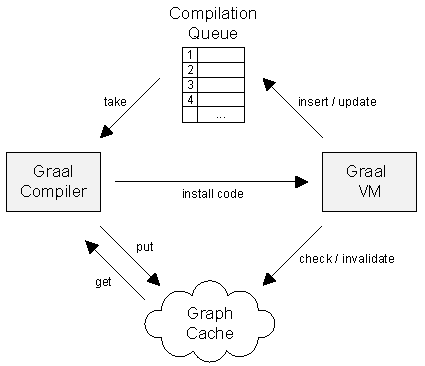
\includegraphics[width=0.75\textwidth]{graal_architecture.pdf}
\end{table}
\end{frame}

\begin{explainframe}{Graal VM - Details}
\begin{enumerate}
    \item HotSpot VM detects \textit{hot} methods
    \item HotSpot VM adds these methods to compilation queue
    \item Compiler threads compile methods with highest priorities
    \item Machine code is installed into runtime's cache
\end{enumerate}
\end{explainframe}



\section{Truffle in Practice}

\begin{frame}{Ways to use Truffle within an existing AST Interpreter}

\begin{description}
 \item[Convert to Truffle:] Port all AST Nodes to Truffle nodes
 \item[Add-on Truffle:] Add an additional set of AST nodes:

\begin{table}
    \centering
    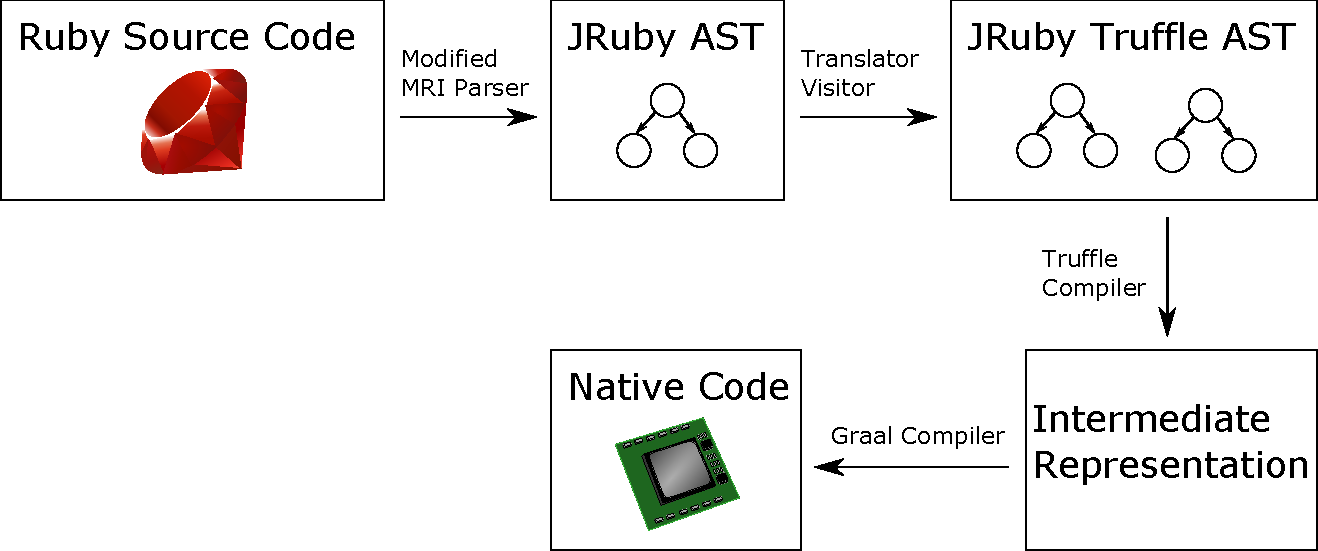
\includegraphics[width=0.75\textwidth]{graaltruffle.pdf}
\end{table}
\end{description}
\end{frame}

\begin{frame}{Method Call Nodes in (J)Ruby}
\begin{table}
    \centering
    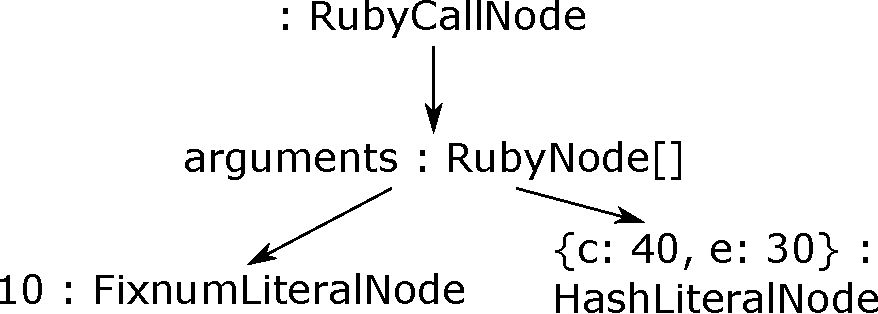
\includegraphics[width=0.75\textwidth]{kwarg_1.pdf}
\end{table}

\begin{itemize}
    \item Call Node contains:
      \begin{itemize}
      \item receiver object
      \item method name (fix)
      \item list of argument AST nodes
      \item block AST node
      \end{itemize}
    \item Dynamic call $\rightarrow$ dynamic dispatch is run on every execution
\end{itemize}
\end{frame}

\begin{frame}{Method Callee Node in (J)Ruby}
\begin{enumerate}
 \item RubyRootNode
 \item Catch*Nodes (CatchNextNode, CatchRetryAsErrorNode, CatchReturnNode \dots)
 \item SequenceNode \begin{enumerate}
    \item CheckArityNode
    \item WriteFactory for args 1
    \item WriteFactory for args 2
    \item WriteFactory for kw e
    \item WriteFactory for kw c
    \item statement sequence itself (wrapped in TracingNodes, with CyclingAssumptions)
  \end{enumerate}
\end{enumerate}
Nice: every argument has a Node to create its default argument, maybe a Node that throws every time a exception
\end{frame}



\section{Challenge: Optimize Keyword Arguments in JRuby}

\begin{frame}[fragile]{Task: Keyword Arguments in Ruby 2.x}

\begin{itemize}
 \item Shortcut to call method with dictionary as last argument:
    \begin{lstlisting}
    method(10, e: 30, c: 40)
    method(10, {:e => 30, :c => 40})
    \end{lstlisting}
  \item Starting with Ruby 2.0 Ruby can process this dictionary automatically (keyword arguments):
    \begin{lstlisting}
    def method(a, b=3, e:, c:30)
    end
    \end{lstlisting}
\end{itemize}
\end{frame}

%\begin{frame}{First Optimizations}
%\begin{itemize}
% \item Reduce duplicate method calls
% \item Using iterators to improve RubyHash handling
%\end{itemize}
%\end{frame}

\subsection{Problem}

\begin{frame}{Performance Bottlenecks}
\begin{itemize}
    \item \lstinline{Hash} object creation: object is created, passed as argument, then destructed again
    \item Inefficient code paths (e.g., multiple scans of \lstinline{Hash} object)
    \item Code involving \lstinline{Hash} objects is harder to optimize than code involving primitive objects (Graal optimizations)
    \item Keyword argument nodes are not optimized by Truffle (Java \lstinline{equals}, Truffle boundary for \lstinline{Hash} iterator)
\end{itemize}

\begin{table}
    \centering
\textbf{Goal: pass keyword arguments like normal arguments}
\end{table}
\end{frame}


\subsection{Solution}
\begin{frame}{Store Keyword Arguments in Array}
\begin{itemize}
    \item Before: \lstinline{RubyCallNode.arguments} contains a \lstinline{Hash} as last array element
    \item Idea: add key-value pairs to array with marker object as hash separator
    \item Benefit: no \lstinline{Hash} creation
\end{itemize}
\end{frame}

\begin{frame}{Store Keyword Arguments in Array}{AST: \lstinline{RubyCallNode} arguments}
\begin{table}
\begin{tabular}{|c|c|c|c|c|c|c|c|c|c|}
\hline
$\mathit{arg}_1$ & \ldots & $\mathit{arg}_{n-1}$ & * & $\mathit{key}_1$ & $\mathit{value}_1$ & $\mathit{key}_2$ & $\mathit{value}_2$ & \ldots & * \\
\hline
\end{tabular}
\end{table}
\begin{itemize}
    \item $\mathit{arg}_i$: $i$th argument (\lstinline{RubyNode})
    \item *: marker (\lstinline{MarkerNode}, executes to singleton \lstinline{Object})
    \item $\mathit{key}_i$: $i$th key in \lstinline{Hash} (\lstinline{StringLiteralNode})
    \item $\mathit{value}_i$: $i$th value in \lstinline{Hash} (\lstinline{RubyNode})
\end{itemize}
\end{frame}

%\begin{frame}{Store Keyword Arguments in Array}{Arguments (objects) in Method Execution}
%\begin{table}
%\begin{tabular}{|c|c|c|c|c|}
%\hline
%method & declarationFrame & self & block & countKwArgs  \\
%\hline
%\end{tabular}
%\end{table}
%\begin{table}
%\begin{tabular}{|c|c|c|c|c|}
%\hline
% $\mathit{arg}_0$ & \ldots & $\mathit{arg}_{n-1}$ & *  & $\mathit{key}_1$\\
%\hline
%\end{tabular}
%\end{table}

%\begin{table}
%\begin{tabular}{|c|c|c|c|c|}
%\hline
% $\mathit{value}_1$ & \ldots  & $\mathit{key}_m$ & $\mathit{value}_m$ & * \\
%\hline
%\end{tabular}
%\end{table}
%
%\begin{itemize}
%    \item $\mathit{arg}_i$: $i$th argument (\lstinline{Object})
%    \item *: marker (singleton \lstinline{Object})
%    \item $\mathit{key}_i$: $i$th key in Hash (\lstinline{String})
%    \item $\mathit{value}_i$: $i$th value in Hash (\lstinline{Object})
%\end{itemize}
%\end{frame}

\begin{frame}{Store Keyword Arguments in Array}
\begin{itemize}
    \item Read keyword argument: scan expanded \lstinline{Hash} or extract value from \lstinline{Hash}.
    \item Read argument: if last argument is expanded \lstinline{Hash}: \\ generate \lstinline{Hash} object.
    \item Read rest keyword arguments: generate \lstinline{Hash} object for keywords that are not excluded.
\end{itemize}
\end{frame}

\begin{frame}{Recap: Type Decision Chains}
\begin{table}
    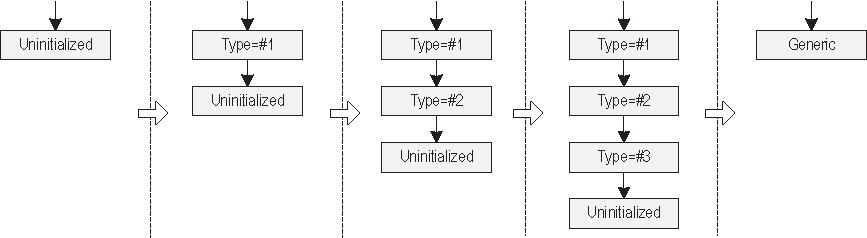
\includegraphics[width=\textwidth]{type_chain.pdf}
\end{table}
\end{frame}

\begin{frame}{Fully Optimized Keyword Arguments}
\begin{itemize}
    \item Before: \lstinline{RubyCallNode.arguments} contains keys and values of keyword arguments
    \item Idea: call node is method-specific and stores values only (no keys!) for arguments specified in signature
    \item Benefit: no linear scan of keyword argument array section
\end{itemize}
\end{frame}

\begin{frame}[fragile]{Fully Optimized Keyword Arguments (Example)}
\begin{lstlisting}
class Cls1
    def method(a:, **kwargs)
    end
end

def Cls2
    def method(a:, b:)
    end
end

def getObject
    # first call returns "Cls1.new"
    # second call returns "Cls2.new"
end

2.times do
    getObject().method(a: 1, b: 2)
end
\end{lstlisting}
\end{frame}

\begin{frame}{Fully Optimized Keyword Arguments (Example)}{Type Decision Chain}
\begin{table}
    \centering
    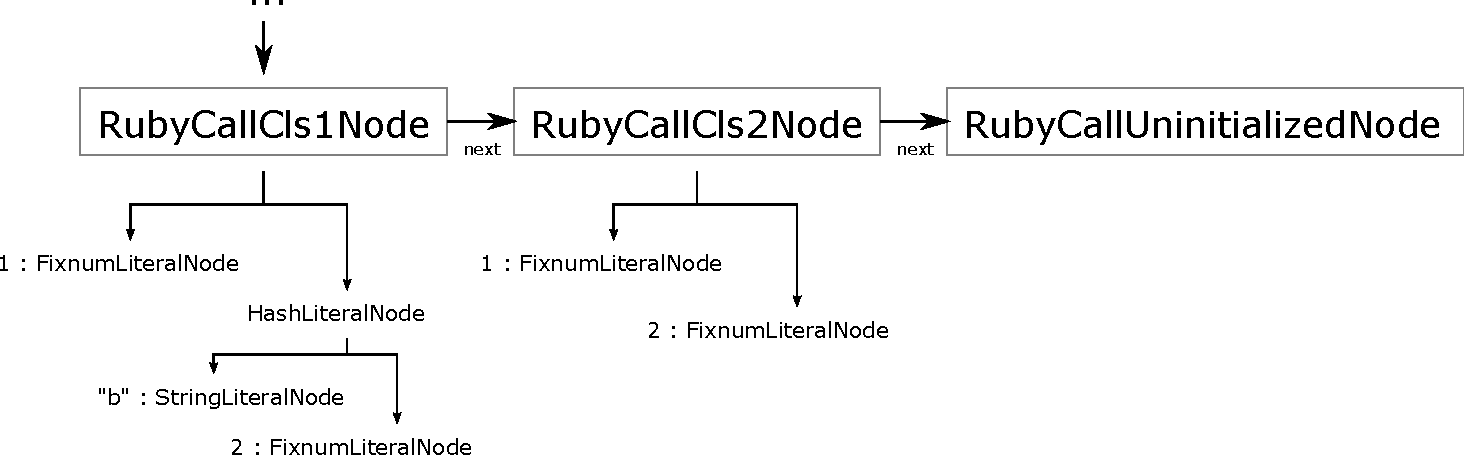
\includegraphics[width=\textwidth]{fully_opt.pdf}
\end{table}

\begin{itemize}
    \item Node specialization for every method (for every receiver type)
    \item Specialized nodes do not construct \lstinline{Hash} nodes only to read arguments from them
\end{itemize}
\end{frame}

\begin{frame}{Fully Optimized Keyword Arguments (Example)}{Generic Case}
\begin{table}
    \centering
    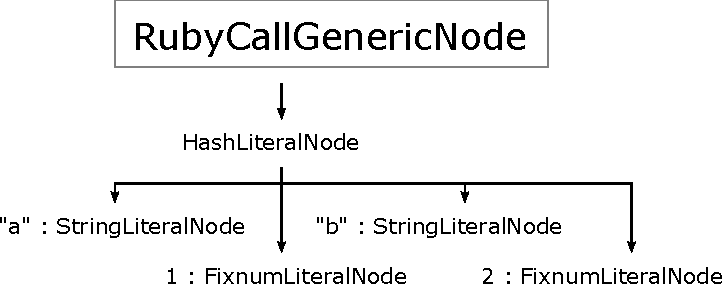
\includegraphics[width=\textwidth]{kwargs_generic.pdf}
\end{table}
\end{frame}

\begin{frame}{Fully Optimized Keyword Arguments}{Problems}
\begin{itemize}
    \item Nodes are specific with regard to user-defined Ruby classes \\ (cannot use Truffle DSL)
    \item Specializations are defined in Java code \\ (need to generate Java classes on the fly)
    \item Type of receiver is not known before dispatching the call
\end{itemize}
\end{frame}

\begin{frame}[fragile]{Polymorphic Inline Caching in Truffle}
\begin{itemize}
    \item Supported by Truffle via type decision chains for types that are known at guest language implementation compile time
    \item Not supported by Truffle for types defined in guest language
    \item Example: Guest language PIC in JRuby
\end{itemize}

\begin{table}
\begin{lstlisting}
@TypeSystem({
    boolean.class,
    byte.class,
    int.class,
    long.class,
    float.class,
    String.class,
    RubyBignum.class,
    RubyArray.class,
    RubyHash.class,
    RubyModule.class, ... })
\end{lstlisting}
\end{table}
\end{frame}

\begin{frame}{Guest Language PIC in JRuby}
\begin{table}
    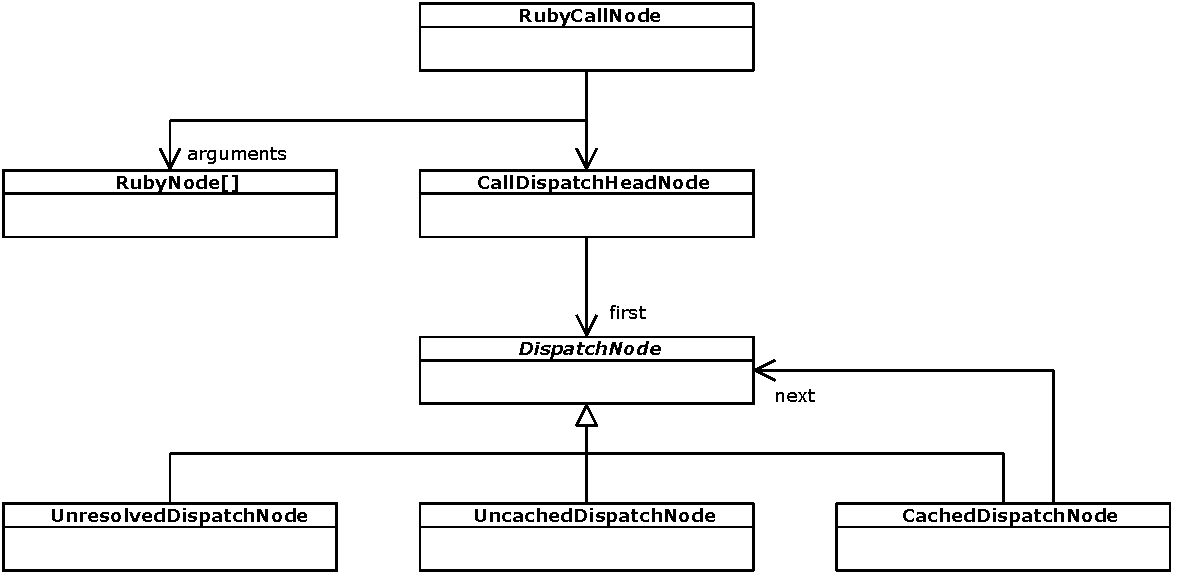
\includegraphics[width=\textwidth]{dispatch.pdf}
\end{table}
\end{frame}

\begin{explainframe}{Guest Language PIC in JRuby}
\begin{itemize}
    \item \lstinline{UnresolvedDispatchNode}: corresponds to Truffle's \emph{unspecified node}
    \item \lstinline{UncachedDispatchNode}: corresponds to Truffle's \emph{generic node}
    \item \lstinline{CachedDispatchNode}: corresponds to Truffle's \emph{specialized nodes}
    \item Node rewriting similar to Truffle but without Truffle
\end{itemize}
\end{explainframe}

\begin{frame}{Argument Passing in \lstinline{DispatchNode}}
\begin{table}
    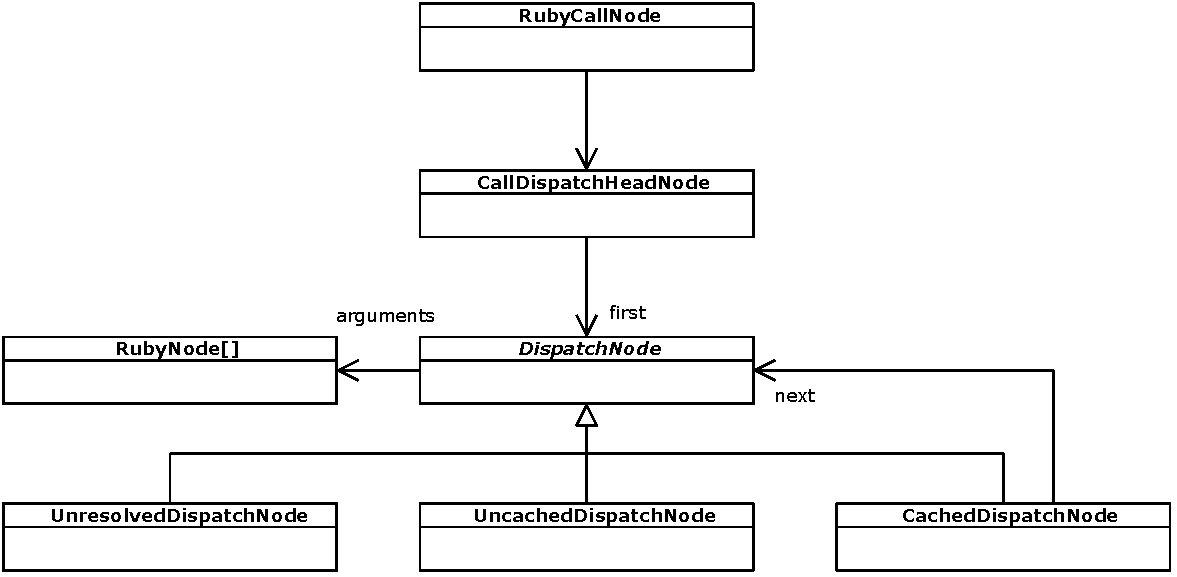
\includegraphics[width=\textwidth]{dispatch_opt.pdf}
\end{table}
\end{frame}

\begin{explainframe}{Argument Passing in \lstinline{DispatchNode}}
\begin{itemize}
    \item Unmodified arguments array (possible with \lstinline{HashLiteralNode}) is stored in \lstinline{UnresolvedDispatchNode}
    \item \lstinline{CachedDispatchNode} contains keyword arguments mentioned in signature in array, and other keyword arguments in \lstinline{HashLiteralNode}
    \item \lstinline{ReadKeywordArgumentNode} checks if method dispatch is optimized (marker present in arguments array) and reads keyword arguments from arguments array, otherwise extracts them from \lstinline{Hash} (same as before)
\end{itemize}
\end{explainframe}

\begin{frame}{Evaluation}
benchmarks and explain why it is faster

\begin{itemize}
    \item Optimization affects only arguments passed in keyword argument syntax in method calls
    \item Optimization does not affect keyword arguments passed as an already existing \lstinline{Hash}
\end{itemize}
\end{frame}

\section{Summary}
%%%%%%%%%%%%%%%%%

\begin{frame}{Truffle Summary}
\begin{itemize}
 \item Specific java code cannot be translated by graal (or it is disallowed)
 \item Large AST interpreter can still be get unclear/distracting (it is java $\rightarrow$ some code needed to get things done)
 \item It is still needed to write efficient code / node implementations
\end{itemize}
\end{frame}

\begin{frame}{Truffle and RPython - a Very Subjective Comparison}
\begin{description}
 \item[RPython] \begin{itemize}
  \item lightwight stack
  \item a little bit easier to get to work - mostly getting the correct libs in the python path
  \item difficult to debug in depth what is happening at execution
\end{itemize}
\item[Truffle] \begin{itemize}
  \item heavy stack (java, mostly multiple JDK and often maven \dots)
  \item if you get it working, you have the full power of (debugging) java, even graal itself
\end{itemize}
\end{description}
\end{frame}
\end{document}
